\documentclass[a4paper,10pt]{article}

% --- TIMES NEW ROMAN & ATS ENCODING ---
\usepackage[T1]{fontenc}
\usepackage{times}

\usepackage[a4paper,margin=0.40in]{geometry}
\usepackage{enumitem}
\usepackage{titlesec}
\usepackage[hidelinks]{hyperref}
\usepackage{graphicx}

% Clean, tight spacing for section headings
\titleformat{\section}{\large\bfseries}{}{0em}{}[\titlerule]
\titlespacing*{\section}{0pt}{5pt}{4pt}

% Globally reduce itemize vertical heights (pointers height reduction)
\setlist[itemize]{
    noitemsep,
    topsep=1pt,
    parsep=0pt,
    partopsep=0pt,
    itemsep=1.5pt
}

\setlength{\parindent}{0pt}

\begin{document}
\pagestyle{empty}

% HEADER
\begin{minipage}[t]{0.75\textwidth}
    {\LARGE \textbf{ATHARVA SURAJ SONAWANE}}\\[4pt]
    {\Large \textbf{Full Stack Developer}}\\[6pt]
    \textbf{Phone:} +91-8378040415\\
    \textbf{Email:} \href{mailto:atharva.sonwane04@gmail.com}{atharva.sonwane04@gmail.com}\\[4pt]
    \textbf{Location:} Pune, 411004\\
    \textbf{Links \& Profiles:}\\
    \href{https://github.com/}{Github}\\
\end{minipage}%
\begin{minipage}[t]{0.25\textwidth}
    \vspace{-10pt}
    \raggedleft
    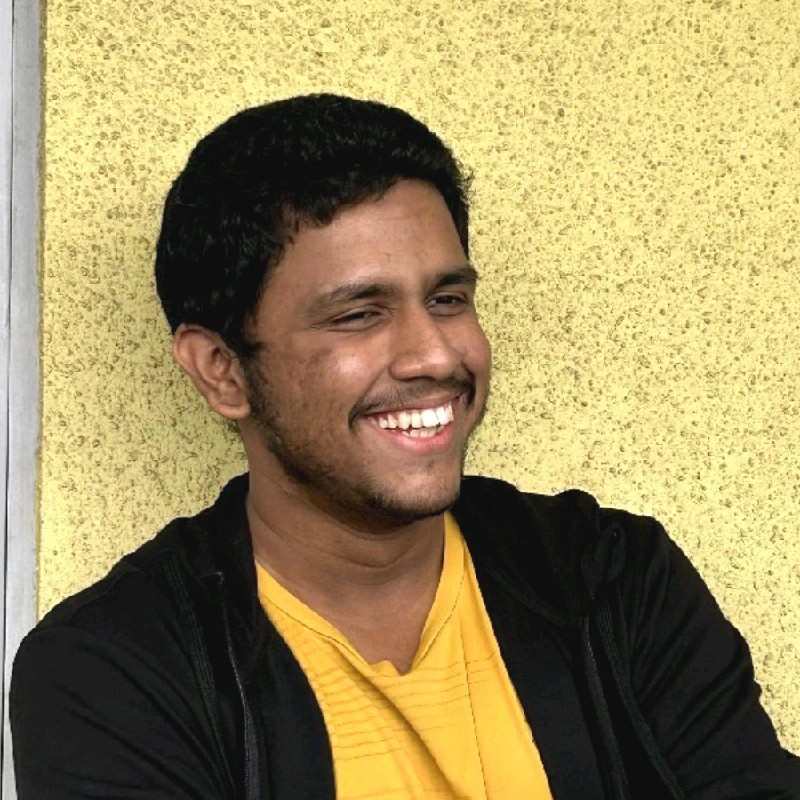
\includegraphics[width=3cm]{../../as.jpg}
\end{minipage}

\vspace{5pt}

\section*{Summary}
Motivated Full Stack Developer currently pursuing a post-degree in MCA at IMCC. Skilled in front-end technologies like HTML, CSS, JavaScript, React, and back-end development with Node.js, Express, and databases like MySQL and MongoDB. I have hands-on experience with Kotlin and knowledge of Flutter, Golang enabling me to develop seamless mobile applications alongside web platforms. Proficient in Git and eager to apply academic knowledge in realworld projects. Passionate about building responsive, scalable web applications and continuously learning new technologies.

\section*{Technical Skills}
\textbf{Frontend Development:}\\[2pt]
HTML, CSS, JavaScript, React.js, Tailwind CSS, Redux, Redux Toolkit, React Router, UI/UX, Vite, CRA, Responsive Web Design, Flutter

\vspace{4pt}
\textbf{Backend Development:}\\[2pt]
Node.js, Express.js, REST API Design (Validation, Pagination, Filtering), JWT Authentication, RBAC, Secure Session Handling, PostgreSQL, MongoDB (Indexing, Query Optimization), Async Processing, Non-blocking I/O

\vspace{4pt}
\textbf{Infrastructure and Tools:}\\[2pt]
AWS (EC2, S3, lambda basics), Git, Linux, Postman, CI/CD basics, Agile (Scrum, Jira)

\section*{Projects}

\textbf{MUSEBEAT - MUSIC APP}\\
\vspace{-6pt}
\begin{itemize}
    \item Developed MuseBeat, a feature-rich music streaming Android application inspired by Spotify.
    \item Integrated ExoPlayer for seamless, high-quality audio playback.
    \item Followed MVVM architecture using ViewModel, LiveData, and Repository for clean code and scalability.
    \item Designed a modern, user-friendly UI using Material Design principles.
\end{itemize}

\vspace{6pt}

\textbf{SkillSync}\\
\vspace{-6pt}
\begin{itemize}
    \item Built SkillSync, a web-based internship recommendation platform that matches students to relevant opportunities using a skill-based intelligent matching algorithm.
    \item Designed a verified student profiling system with admin validation to ensure authenticity and improve the quality of internship recommendations.
    \item Developed a decision-support system for first-time internship seekers, simplifying discovery and reducing mismatched applications through personalized recommendations.
\end{itemize}

\vspace{6pt}

\textbf{JOBJET}\\
\vspace{-6pt}
\begin{itemize}
    \item Developed a full-stack job portal using React.js, Node.js, Express.js, and JWT authentication for secure user sessions.
    \item Designed a responsive UI with Tailwind CSS and optimized file uploads with Multer.
    \item Improved page load times by 40\% and reduced development time by 50\% with the chosen tech stack.
    \item Enhanced performance by minimizing error rates and speeding up form validation for a smoother user experience.
\end{itemize}

\section*{Experience}
\textbf{Software Developer} $|$ \textit{SITRAMIX, Pune} \hfill May 2025 -- December 2025
\begin{itemize}
    \item Designed and developed 20+ RESTful API endpoints using Node.js and Express with validation, pagination, and structured error handling.
    \item Implemented JWT-based authentication and RBAC to enforce secure access control across multiple user roles and protected routes.
    \item Optimized database queries and indexing strategies, reducing API response time by $\sim$20--30\% under typical load conditions.
    \item Handled concurrent requests using async patterns, supporting 100+ requests/minute with non-blocking execution.
    \item Designed API contracts and response structures to ensure consistency and scalability across services.
    \item Structured backend architecture for maintainability, including middleware usage, request lifecycle control, and modular routing.
    \item Deployed and monitored backend services on AWS, contributing to stable production releases.
    \item Collaborated with frontend systems by designing clean API contracts and consistent response structures.
\end{itemize}

\section*{Education}
\textbf{Masters in Computer Application (MCA)}  \hfill 2025 -- 2027 \quad \textbf{Percentage: 80.96\%}

\vspace{4pt} 

\textbf{Bachelor in Business Administration in Computer Application (BBA-CA)}  \hfill 2022 -- 2025 \quad \textbf{Percentage: 85.04\%}

\vspace{4pt} 

\textbf{12th Class Higher Secondary Education (H.S.C)}  \hfill 2021 -- 2022 \quad \textbf{Percentage: 65.33\%}

\vspace{4pt} 

\textbf{10th Class Secondary Education (S.S.C)}  \hfill 2019 -- 2020 \quad \textbf{Percentage: 78.40\%}

\end{document}
